\chapter{LoRa et LoRaWAN}

Il existe deux couches distinctes dans l’écosystème LoRa, premièrement il y a la couche physique LoRa et ensuite la couche protocolaire LoRaWAN, parfois également appelé LoRa MAC.

La couche LoRa est une couche physique qui définit le type de modulation utilisé pour envoyer les données brute grâce à des ondes électromagnétiques. Cette couche n’a pas la connaissance des hautes couches et peut donc être utilisé avec n’importe quel protocole.

La couche LoRaWAN quant à elle est une couche protocolaire MAC qui s’appuie sur la couche physique LoRa. Elle définit les aspects réseaux comme la topologie employée, le moyen de relayer les messages entre les acteurs ainsi que les aspects sécuritaires comme le chiffrement des données.

Il est possible de n’utiliser que la couche physique LoRa sans le LoRaWAN, ceci simplifie beaucoup le système par contre cela implique la perte d’un certain nombre de fonctionnalité qui sont proposées par le protocole.

Le choix ou non d’utiliser la couche protocolaire LoRaWAN est détaillé à la fin du chapitre.

\section{La couche physique LoRa}

La couche physique LoRa définit de quelle manière les données sont transformées pour être transmise par des ondes radios. La technique de modulation de base pour transformer les informations en signal se porte sur le principe d’étalement de spectre (spread spectrum), l’idée est d’étaler les données sur une largeur de spectre plus grande que le signal en modifiant la phase de la fréquence porteuse du transmetteur en suivant une séquence pseudo aléatoire.

L’avantage de la technique de l’étalement de spectre réside dans le fait que les signaux émis sont par définition plus résistant aux interférences externes que si le signal était transmis normalement. Le Direct Sequence Spread Spectrum est une technique de modulation qui applique ce principe. Cette technique est beaucoup utilisée, notamment par la norme 802.11b (WiFi). Le prix a payé pour utiliser cette méthode est qu’elle nécessite la présence d’une horloge très précise sur le récepteur et le transmetteur afin de pouvoir coder et décoder les signaux correctement. En plus l’opération en elle-même est également un processus qui prend passablement de temps et de ressource et qui dépend de la séquence de codage utilisée. Ses aspects font que le Direct Sequence Spread Spectrum n’est pas approprié pour des applications à bas coût et basse consommation comme ceux requis pour ce projet.

La couche physique LoRa vise à corriger ses défauts en utilisant également une méthode d’étalement de spectre un peu différente que le Direct Sequence Spread Spectrum. Elle se base sur une autre technique nommée Chirp Spread Spectrum. Cette technique a été développée dans les années 1940 pour être employé dans les radars. L’étalement de spectre est toujours un élément central cependant la séquence pseudo aléatoire a été abandonnée ce qui simplifie la gestion de la modulation et permet à des équipements basse consommation de l’utiliser sans contrepartie coûteuse. \cite{lora_modulation_basics}

La technique de modulation utilisé par la couche physique Lora se nomme logiquement LoRa Spread Spectrum, elle utilise la bande de fréquence libre Industrielle, scientifique et médicale (ISM) qui, pour l’Europe, utilise la bande de fréquence 868 Mhz. Cette bande de fréquence n’est pas soumise à autorisation pour être utilisée, ce qui est donc un avantage de taille et qui limite les coûts supplémentaires. Cette modulation permet au moyen de paramètre changeable, des débits de transferts allant de 0.3 kbps à 27 kbps, suivant le débit sélectionné on pourra envoyer plus ou moins de donnés, entre 51 à 222 octets par message. \cite{limits_lorawan}

\section{La couche MAC LoRaWAN}

La couche radio LoRa est une technique propriétaire de la société Semtech, cependant la couche protocolaire LoRaWAN qui fait partie du groupe des Low-Power Wide-Area Network (LPWAN), est entièrement ouverte et son standard ainsi que ses évolutions sont gérés par la LoRa Alliance qui est une association qui regroupe diverses entreprises ou groupes qui sont actifs dans le domaine des communications sans fils.

Le protocole LoRaWAN définit les acteurs qui font partis du réseau. Ils sont décrits dans la figure ~\ref{fig:schema_lorwan} .

\begin{figure}[htb]
\centering 
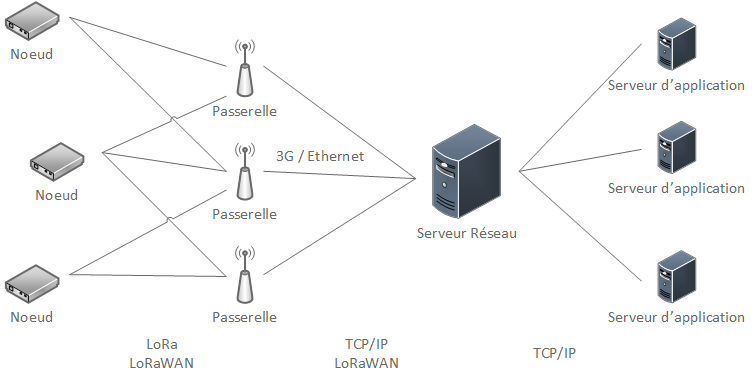
\includegraphics[width=1\columnwidth]{../images/schema_lorawan.png} 
\caption[Architecture des réseaux LoRaWAN]{Architecture des réseaux LoRaWAN}
\label{fig:schema_lorwan}
\end{figure}

Les aspects sécuritaires, à travers l’utilisation de la cryptographie symétrique, la définition des procédures pour rejoindre le réseau et la gestion des taux de transferts des nœuds sont également des éléments abordés dans ce standard. Un des aspects intéressant du LoRaWAN est qu’il peut employer une technique appelé Adaptative Data Rate (ADR) qui est une façon de maximiser la vie des batteries des nœuds et la capacité du réseau en donnant la possibilité à l’infrastructure du réseau LoRaWAN de changer le taux de transfert et la fréquence de transmission pour chaque nœud individuellement. Cela permet au réseau de diminuer le taux de transferts d’un nœud très éloigné tout en augmentant son facteur d’étalement, ce qui fera qu’il prendra plus de temps à envoyer les données mais elles auront plus de chance de parvenir jusqu’à la passerelle, inversement les nœuds proches auront leur taux de transfert augmenté mais leur facteur d’étalement diminué.

La figure ~\ref{fig:layers_lorawan}  montre l’architecture d’une application utilisant le LoRaWAN.

\begin{figure}[htb]
\centering 
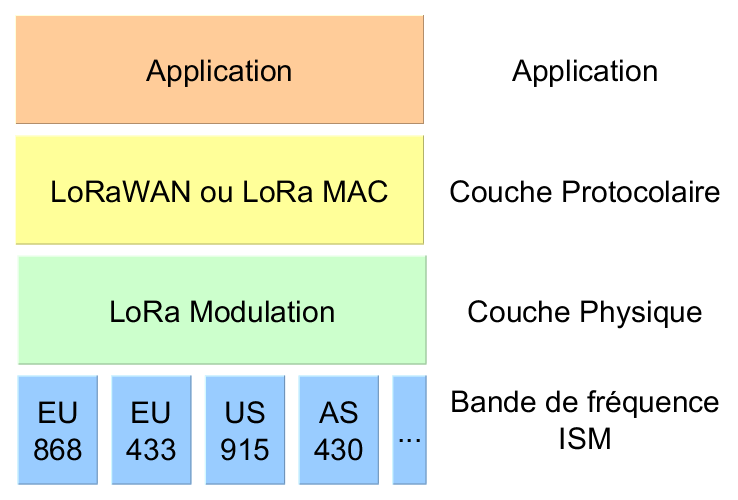
\includegraphics[width=0.7\columnwidth]{../images/lora_layers.png} 
\caption[Couches LoRa]{Couches LoRa – Document LoRaWAN Specification v1.1}
\label{fig:layers_lorawan}
\end{figure}

C’est également dans ce standard qu’est définie l’architecture du réseau dans son ensemble, c’est-à-dire comment les données sont acheminées d’un nœud jusqu’au serveur réseau qui traite et stock les données. Les données sont acquises par le nœud et ensuite transmise à la couche LoRaWAN qui les envoie grâce à la couche radio LoRa. Une fois le paquet reçu par la passerelle, un packet forwarder est en charge de l’envoyer à destination du serveur réseau, généralement en utilisant le protocole UDP. Le serveur réseau est ensuite responsable de la gestion du protocole LoRaWAN, c’est lui, si nécessaire, qui génère les acquittements des paquets et les retransmets à une passerelle pour être envoyé au nœud. Enfin le serveur réseau transmets les données utiles reçus des nœuds aux serveurs d’application qui vont les exploiter pour par exemple montrer l’évolution de la température dans une région ou encore la position d’un élément mobile. \cite{lorawan_spec}

La figure ~\ref{fig:network_lorawan}  montre l’architecture d’un réseau LoRaWAN dans son ensemble ainsi que le détails de chaque éléments.

\begin{figure}[htb]
\centering 
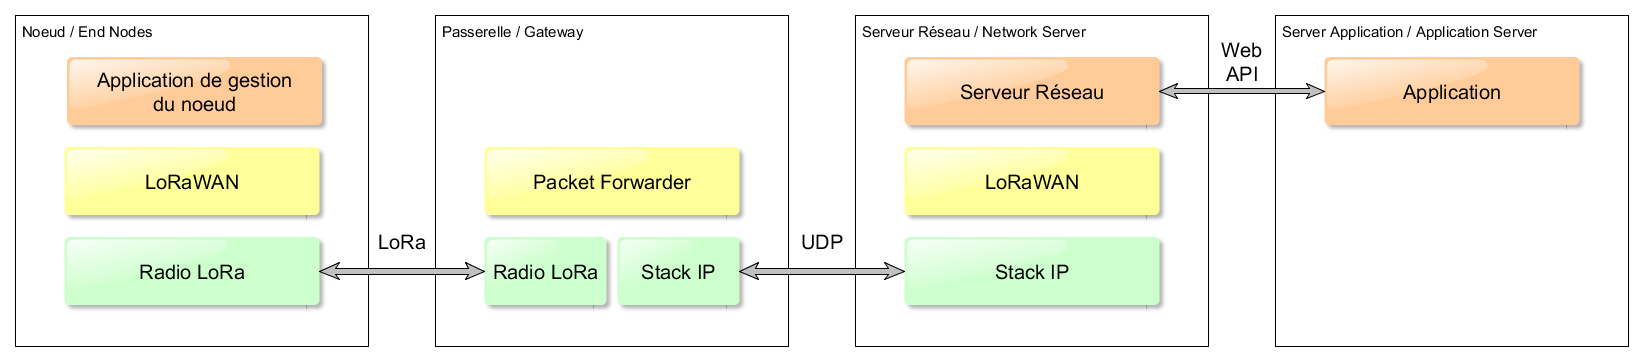
\includegraphics[width=1\columnwidth]{../images/lorawan_reseau.png} 
\caption[Eléments d'un réseaux LoRaWAN]{Eléments d'un réseaux LoRaWAN}
\label{fig:network_lorawan}
\end{figure}

\section{Utilisation de LoRaWAN}

La couche protocolaire LoRaWAN offre beaucoup d’avantage cependant elle nécessite énormément de travail pour être entièrement mise en place pour un réseau privé comme c’est le cas dans ce projet. Dans le cas où un nombre important de nœuds ainsi que plusieurs passerelles sont exploités, cette couche prend tout son sens car elle offre des moyens de gestion de l’ensemble du réseau et permet de centraliser l’information. Elle offre également une interface web moderne qui permet la récupération des données produite par les nœuds afin de les exploiter dans de diverses applications. Elle s’occupe aussi de la gestion du chiffrement des données transmises par les nœuds jusqu’aux passerelles par exemple.

Dans le cadre du travail de Bachelor et dans un esprit de simplification, la couche LoRaWAN ne sera pas utilisée. Comme expliqué elle nécessite la mise en place d’une infrastructure réseau complexe ce qui complique passablement la mise au point du projet. Il est clair que dans une optique de développement d’un produit, ce protocole prendrait tout son sens mais le développement du prototype mais l’accent sur la définition du système, principalement du capteur, ainsi que des logicielles associés. L’utilisation d’un serveur hébergé sur internet rajoute également de la complexité au niveau de la passerelle, puisque le système sera testé en extérieur, cela nécessite l’ajout d’une interface de communication par le réseau mobile, 3G par exemple, afin de pouvoir transmettre les données récoltées par la passerelle au serveur. Enfin, puisque le prototype ne sera composé que d’un seul capteur et d’une seule passerelle, l’utilisation du protocole LoRaWAN n’apporte que très peu d’avantage au prix d’une complexité accrue.

Afin de pouvoir concentrer le travail sur le développement du capteur, de la passerelle et de l’application mobile, il semble judicieux de ne pas se lancer dans la mise en place longue et coûteuse que représente l’utilisation du LoRaWAN. Néanmoins, dans une optique d’évolution du projet, le développement durant le travail de Bachelor sera pensé de façon à faciliter l’éventuelle modification ultérieure du système afin de pouvoir utiliser le protocole LoRaWAN.
